 \subsection{Симплициальные гомологии}

    \begin{definition}
        \emph{Цепным комплексом} абелевых групп $(C_{\bullet}, \partial)$ называется последоватекльность абелевых групп и морфизмов вида
        \[ \ldots \xrightarrow{ \partial_{q + 2}} C_{q + 1} \xrightarrow{\partial_{q + 1}} C_{q} \xrightarrow{\partial_{q}} \ldots, \quad \text{ где } C_{i} \text{~--- абелевы группы} \]
        при условии $\partial_{q} \circ \partial_{q + 1} = 0$. Если комплекс обрывается с одной из сторон, то мы считаем, что он дополнен нулями.

        Элементы группы $C_{q}$ называют $q$-мерными цепями, а отображение $\partial$ называют (граничным) дифференциалом.
    \end{definition}

    \begin{remark}
       Ясно, что условие $\partial_{q} \circ \partial_{q + 1} = 0$ равносильно тому, что $\Ker{\partial_{q}} \supset \Im{\partial_{q + 1}}$.
    \end{remark}

    \begin{remark}
       Когда комплекс снабжают отображением $C_0 \xrightarrow{\varepsilon}  \Z$, это отображение называют \emph{аугументацией}.
    \end{remark}


    \begin{definition}
        \emph{Гомологиями} комплекса $(C_{\bullet}, \partial)$ называют абелевы группы
        \[ H_{q}(C_{\bullet}, \partial) \eqdef \Ker{\partial_{q}} / \Im{\partial_{q + 1}}. \]

        Если коплекс снабжен аугументацией и обрывается на нулевом члене, то у него также есть \emph{приведённые гомологии}
        \[ H_{0}(C_{\bullet}, \partial) = C_0/\Im{\partial_{1}}, \quad \widetilde{H_0}(C_{\bullet}, \partial) = \Ker{\partial_{0}}/\Im{\partial_{1}}, \quad \widetilde{H}_{q} = H_{q} \ \forall q > 0, \]
        которые отличаются от обычных только в нулевом члене.
    \end{definition}

    Перед тем как что-то строго определять, посмотрим нестрого на какие-то мотивирующие примеры вычислений. Для этого лучше всего подойдут \emph{симплициальные гомологии}.
    Неформально, идея состоит в том, что мы разбиваем топологическое пространство $X$ на симплексы всех размерностей и говорим, что $C_{q}(X, \Z)$~--- свободная абелева группа, порожденная всеми
    $q$-мерными симплексами (то есть, мы рассматриваем целочисленные формальные линейные комбинации симплексов). Дифференциалом $\partial$ будет оператор взятия границы (топологической).

    \begin{example}[Симплицаильные гомологии отрезка (нестрого)]

        Пусть $X$~--- отрезок $[a, b]$ с ориентацией из $b$ в $a$. В нём две нульмерные клетки, значит $C_0(X, \Z) = \Z^2$, одномерная клетка одна~--- ребро $e$, то есть $C_{1}(X, \Z) = \Z$
        и комплекс устроен следующим образом:
        \[ \ldots 0 \to  C_{1} \xrightarrow{\partial_{1}} C_{0} \xrightarrow{\varepsilon} \Z, \]
        так как мы можем определить аугументацию следующим образом: $x \in C_0 \Rightarrow$ $x = k_1 a + k_2 b$, положим $\varepsilon(x) = k_1 + k_2$.
        То есть, на самом деле комплекс выглядит вот так:
        \[ \ldots \to 0 \to \Z \xrightarrow[e \to \partial e = a - b]{} \Z^{2} \xrightarrow[a \to 1, \ b \to 1]{} \Z.\]
        Заметим, что $\varepsilon \circ \partial = 0$.

        Гомологиями топологического пространства называют гомологии построенного по нему комплекса. В нашем случае
        \[ H_{1}(X, \Z) = \Ker{\partial_{1}}/\Im{\partial_{2}} = 0/0 = 0. \]
        \[ \widetilde{H_{0}}(X, \Z) = \Ker{\varepsilon} / \Im_{\partial_{1}} = \langle a - b \rangle / \langle a - b \rangle = 0. \]
        \[ H_{0}(X, \Z) = C_0(X, \Z) = C_{0}(X, \Z)/\Im_{\partial_{1}} = \Z^2 / \Z = \langle a, b \rangle / \langle a - b \rangle = \langle a \rangle = \Z\]
    \end{example}

    \begin{example}[Симплицальные гомологии треугольника]\label{ex2}
        Рассмотрим треугольник $(a b c)$ с внутренностью $\sigma$, ориентированной против часовой стрелки, и рёбрами $b \xrightarrow{e_1} a$, $c \xrightarrow{e_3} a, c \xrightarrow{e_2} b$.
        \begin{center}
            \begin{tikzpicture}
            \node at (0,0){\includegraphics[scale = 0.7]{lectures/0/pictures/pic_1}};
            \node at (0.1, -0.2){\small \( \sigma \)};
            \node at (-0.9, 0){\small \( e_1 \)};
            \node at (1, 0){\small \( e_2 \)};
            \node at (0, -1.3){\small \( e_3 \)};
            \node at (0.2, 1.3){\small \( b \)};
            \node at (-1.4, -1.25){\small \( a \)};
            \node at (1.4, -1.25){\small \( c \)};
            %	\draw[opacity=0.7] \foreach \x in {-4,...,5} {
	   (\x cm, 0.1) -- (\x cm, -0.1) node[below]{\tiny \x}
	   (\x cm - 0.5cm, 0.08) -- (\x cm - 0.5cm, -0.08)
	   \foreach \t in {1,2,3,4,6,7,8,9} {
	      (\x cm - 0.1 * \t cm, 0.055) -- (\x cm - 0.1 * \t cm, -0.055)
	   }
	};
	\draw[opacity=0.7,rotate=90] \foreach \x in {-3,-2,-1,1,2,3,4} {
	   (\x cm, 0.1) -- (\x cm, -0.1) node[right]{\tiny \x}
	   (\x cm - 0.5cm, 0.08) -- (\x cm - 0.5cm, -0.08)
	   \foreach \t in {1,2,3,4,6,7,8,9} {
	      (\x cm - 0.1 * \t cm, 0.055) -- (\x cm - 0.1 * \t cm, -0.055)
	   }
	};

            \end{tikzpicture}
        \end{center}
        Тогда цепной комплекс, построенный по треугольнику будет устроен следующим образом:
        \[ \ldots \to 0 \to \Z \xrightarrow[\sigma \to e_1 + e_2 - e_3]{\partial_{2}} \Z^3 \xrightarrow{\partial_1} \Z^3 \xrightarrow{\varepsilon} \Z \]
        Из ориентации $\sigma$ ясно, что $\partial \sigma = e_1 + e_2 - e_3, \ \partial e_1 = b - c, \ \partial e_2 = a - b, \partial e_3 = a - c$.
        Ясно, что вторые гомологии нулевые:
        \[ H_{2}(X, \Z) = \Ker{\partial_{2}}/0 = 0\]
        Посчитаем теперь первые.
        \begin{multline*} \partial(k_1 e_1 + k_2 e_2 + k_3 e_3) =  k_1(b - c) + k_2(a - b) + k_3(a - c) = a(k_2 + k_3) + b(k_1 - k_2) + c(-k_1 - k_3) \Rightarrow \\ \Rightarrow \Ker\partial_{1} = \langle (k_1, k_2, k_3) \in \Z^3 \ \vert \ k_1 = k_2 = -k_3 \rangle \end{multline*}
        С другой стороны, $\Im{\partial_{2}} = k(e_1 + e_2 - e_3)$. Тем самым, $H_{1}(X, \Z) = 0$. Аналогичным вычислением мы получаем, что $H_{0}(X, \Z) = \Z$.
    \end{example}

    \begin{example}[Спмилициальные гомологии треугольника без внутренности]
        Пусть теперь всё также, как в примере~\ref{ex2}, но у треугольнка нет внутренности.
        Тогда цепной комплекс будет иметь вид
        \[ \ldots \to 0 \to \Z^3 \xrightarrow{} \Z^3 \xrightarrow{} \Z \]
        Из того, как поменялись отображения, ясно, что поменялись только первые гомологии. Теперь $H_{1}(X, \Z) = \Z/\{ 0 \} = \Z$, а
        образующая~--- это цикл $e_1 + e_2 - e_3$. С другой стороны, $\pi_{1}(\Delta) = \Z$.
    \end{example}

    \begin{remark}
       Когда-нибудь позже мы докажем, что для любого симплициального пространства $X$ есть отображение
        \[ \pi_{1}(X) \to H_{1}(X) = \pi_{1}(X)^{ab} = \pi_{1}(X)/[\pi_{1}(X), \pi_{1}(X)].\]
    \end{remark}

    \begin{example}[Симплициальные гомологии тора $\mathbb{T}^2$]
        Рассмотрим двумерный тор $\mathbb{T}^2$, разбитый на симплексы следующим образом:
        \begin{center}
            \begin{tikzpicture}
            \node at (0,0){\includegraphics{lectures/0/pictures/pic_2}};
            \node at (-0.5, 0.5){\small \( \sigma_1 \)};
            \node at (0.5, -0.5){\small \( \sigma_2 \)};
            \node at (0.2, -0.2){\small \( e_1 \)};
            \node at (-1.5, 0){\small \( e_2 \)};
            \node at (0, -1.4){\small \( e_3 \)};
            %	\draw[opacity=0.7] \foreach \x in {-4,...,5} {
	   (\x cm, 0.1) -- (\x cm, -0.1) node[below]{\tiny \x}
	   (\x cm - 0.5cm, 0.08) -- (\x cm - 0.5cm, -0.08)
	   \foreach \t in {1,2,3,4,6,7,8,9} {
	      (\x cm - 0.1 * \t cm, 0.055) -- (\x cm - 0.1 * \t cm, -0.055)
	   }
	};
	\draw[opacity=0.7,rotate=90] \foreach \x in {-3,-2,-1,1,2,3,4} {
	   (\x cm, 0.1) -- (\x cm, -0.1) node[right]{\tiny \x}
	   (\x cm - 0.5cm, 0.08) -- (\x cm - 0.5cm, -0.08)
	   \foreach \t in {1,2,3,4,6,7,8,9} {
	      (\x cm - 0.1 * \t cm, 0.055) -- (\x cm - 0.1 * \t cm, -0.055)
	   }
	};

            \end{tikzpicture}
        \end{center}
        Из такой триангуляции ясно, что комплекс будет иметь вид:
        \[ \ldots \to 0 \to \Z^2 \xrightarrow{\partial_{2}} \Z^3 \xrightarrow{\partial_{1}} \Z \xrightarrow{\varepsilon} \Z \]
        Посчитаем дифференциал на двумерных клетках: $\partial{\sigma_1} = e_1 - e_3 - e_2, \ \partial{\sigma_{2}} = e_2 + e_3 - e_1$.
        С другой стороны, ясно, что дифференциал зануляется на любой одномерной клетке, $\partial{e_i} = a - a = 0$.
        \[ H_{2}(\mathbb{T}^2,  \Z) = \Ker{\partial_{2}}/0 = \Z. \]
        так как $\partial{\sigma_{1}} = -\partial{\sigma_{2}} \Rightarrow \Ker{\partial_{2}} = \Z$.

        Также прямыми вычислениями можно убедиться, что $H_{1}(\mathbb{T}^2, \Z) = \Z^2 = \pi_1(\mathbb{T}^2)^{ab}$.
        Образующими первых гомологий будут $e_2$ и $e_3$.

        \noindent\bf{Упражнения.}
        \begin{enumerate}
            \item Посчиать по определению одномерные гомологии связного дерева.
            \item Посчитать по определению все гомологии $n$-мерного симплекса $T^n$
                  \[ T^n \eqdef \left\{ (t_0, \ldots, t_n) \ \vert \ t_i \ge 0, \ \sum_{i = 1}^{n} t_i = 1 \right\}.\]
            \item Покажите, что барицентрическое подразбиение не меняет симплициальных гомологий.
        \end{enumerate}

    \end{example}

    Вообще говоря, далее нужно формально доказывать, что гомологии не зависят от симплициального разбиения пространства (и выяснять, у каких пространств это симплициальное разбиение вообще есть),
    но мы этим всем заниматься не будем, так как в нашем курсе основной будет другая теория.

    \subsection{Сигнулярные гомологии}

    \begin{definition}\label{SingHomology}
        Пусть $X$~--- топологическое пространство.
        \begin{itemize}
            \item \emph{Сингулярным $q$-мерным симплексом} мы будем называть непрерывное отображение $f\colon T^{q} \to X$.
            \item Его граница определяется, как формальная линейная комбинация
                    \[ \partial f \eqdef \sum_{i = 0}^{q} (-1)^i \Gamma_i f,\]
                    где $\Gamma_i f$~--- сужение $f$ на грань $t_i = 0$ (сумма именно такая, так как у $q$-мерного симплекса $q + 1$ грань).
            \item \emph{Сингулярными $q$-мерными цепями} $C_{q}(X, \Z)$ мы будем называть формальные целочисленные линейные комбинации конечного числа $q$-мерных сингулярных симплексов (то есть порожденную ими свободную абелеву группу).
            \item Дифферецниал комплекса\footnote{формально, мы пока еще не знаем, что это комплекс.} $C_{\bullet}$ определяется, как продолжение по линейности оператора взятия границы $q$-мерного сингулярного симплекса.
            \item Комплекс сингулярных цепей может быть снабжен аугументацией $\varepsilon \colon C_{0}\to \Z, \ \sum k_i f_i \to \sum k_i$.
        \end{itemize}
    \end{definition}

    \begin{remark}
       Формально говоря, мы пока не знаем, что комплекс из сингулярных цепей~--- это комплекс. Для этого нам понадобится следующая техническая
    \end{remark}

    \begin{lemma}
        В контексте определения~\ref{SingHomology} $\partial^2 = 0$.
    \end{lemma}
    \begin{proof}
        Посчитаем $\partial \partial f$:
        \[ \partial \partial f = \partial \lr*{\sum_{i} (-1)^i \Gamma_i f} =  \sum_{i, j} (-1)^{i + j} \Gamma_{j}\Gamma_{i}f. \]
        Ясно, что любую грань коразмерности 2 можно получить взятием границы двумя способами.
        Действительно, если $j < i$, то $\Gamma_{i}\Gamma_{j} = \Gamma_{j}\Gamma_{i + 1} $ ($i$-я из оставщихся после выкидывания $j$-й координаты~--- $i+1$-я изначально),
        а в сумме слагаемые $\Gamma_{i}\Gamma_{j}$ и $\Gamma_{j}\Gamma_{i + 1}$ будут с разным знаком, значит $\partial \partial f = 0$.
    \end{proof}

    \begin{definition}
        \emph{Сингулярными гомологиями} топологического пространства $X$ называются гомологии комплекса сингулярных цепей. Мы будем обозначать их, как $H_{k}(X)$ или $H_{\textrm{k}}^{\mathrm{sing}}(X)$.

        В топологическом контексте группу $Z_{q}(X) \eqdef \Ker{\partial_{q}}$ часто называют \emph{$q$-циклами}\footnote{позже мы увидим, какая в этом геометрическая интуиция},
        а группу $B_{q}(X) \eqdef \Im{\partial_{q + 1}}$~--- \emph{q-границами}. В этом смысле $H_{q}(X)$~--- циклы с точностю до границ.
    \end{definition}
    
    \begin{remark}
       Из определения очевидно, что сингулярные гомологии зависят только от класса гомеоморфизма пространства $X$ (их основной плюс и состоит в том, что тут это очевидно). 
    \end{remark}


    
